\section{Dynamické parametry obvodů v unipolárních technologiích}
- vstupní, výstupní a převodní charakteristiky, logické obvody ACT, HC, AHC, ALVC. Vliv nízkého napájecího napětí na chování digitálních obvodů
\subsection{Vstupní, výstupní charakteristika}
   \begin{figure}[h]
   \begin{center}
     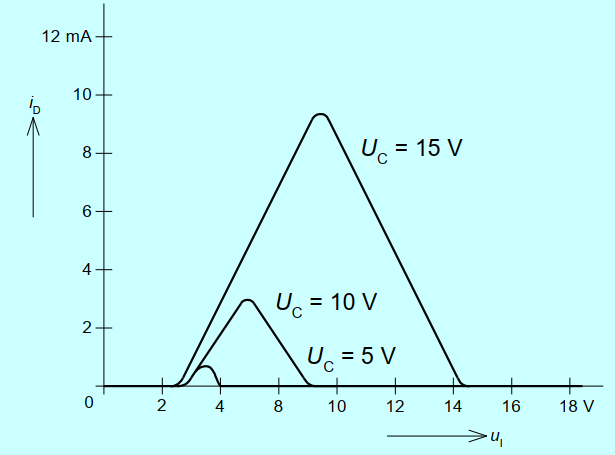
\includegraphics[scale=0.6]{images/VstupCMOS.png}
   \end{center}
   \caption{Proudový odběr hradla v závislosti na vstupním napětí}
  \end{figure}

   \begin{figure}[h]
   \begin{center}
     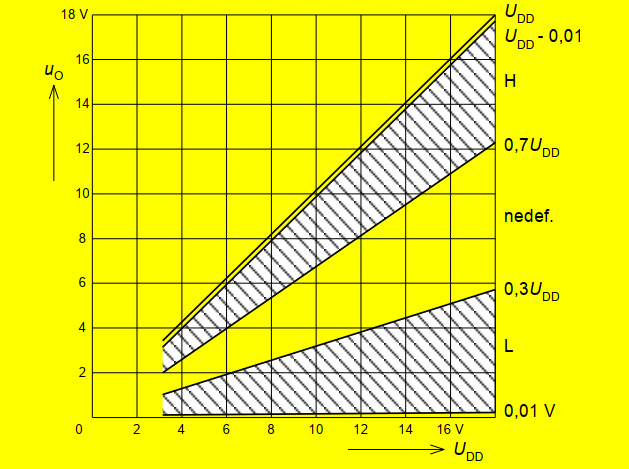
\includegraphics[scale=0.6]{images/VystupCMOS.png}
   \end{center}
   \caption{Překrytí úrovní vstupních a výstupních napětí pro přípustné hodnoty
napájecích napětí}
  \end{figure}



\subsection{Převodní charakteristika}
Tvar těchto charakteristik je podmíněn postupným přechodem tranzistoru T1 z
aktivní oblasti jeho výstupních charakteristik (vějířovitě se rozbíhající soustava
charakteristik v okolí počátku souřadnic, vyznačujících se velkou strmostí) přes
oblast proudové saturace (téměř přímkové charakteristiky, prakticky rovnoběžné s
osou napětí) do stavu zahrazení (charakteristika splývající s osou napětí -
tranzistorem teče jen zbytkový proud) a souběžně probíhajícím přechodem
tranzistoru T2 ze stavu zahrazení přes oblast saturace do aktivní oblasti.
K otevření tranzistoru s kanálem typu N je třeba přivést na jeho hradlo kladné napětí
UGSN převyšující jeho prahové napětí UPN.

Tranzistor s kanálem typu P se otevírá záporným napětím hradla vzhledem k jeho
emitoru U
GSP , toto napětí musí být zápornější, než prahové napětí tranzistoru UPP.

   \begin{figure}[h]
   \begin{center}
     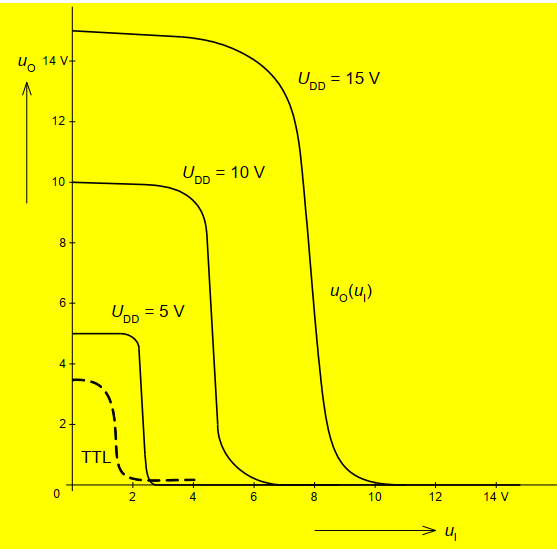
\includegraphics[scale=0.6]{images/PrevodCMOS.png}
   \end{center}
   \caption{Převodní charakteristika pro různá napájecí napětí}
  \end{figure}
  
\subsection{ACT}
Logické obvody AC/ACT – Advanced CMOS Logic jsou vyrobeny v technologii
CMOS 1 $\mu$m. Obvody typu ACL vynikají nízkou spotřebou, ale zároveň jsou schopné
pracovat s výstupním proudem až 24 mA. Vstupy technologie AC jsou kompatibilní
s CMOS logikou a ACT umožňuje navázání obvodů v klasické logice TTL. Řada
74AC představuje skupinu rychlých obvodů CMOS se vstupními úrovněmi CMOS a
posílenými výstupy CMOS, které mohou budit zátěž proudy až ± 24 mA. Doba
zpoždění signálu tp je stejná nebo kratší než u obvodů ALS TTL, avšak mají až
trojnásobně vyšší hodinový kmitočet. Tyto obvody se vyznačují velkou odolností vůči
parazitní kapacitě zátěže

\textbf{Typické vlastnosti těchto obvodů jsou:}\\
\begin{itemize}
\item velmi nízká spotřeba,
\item typické zpoždění 5 ns,
\item napájecí napětí 1,5 V až 5,5 V (AC) a 4,5 V až 5,5 V (ACT),
\item výstupní proud (max.) 24 mA,
\item HC/HCT – High-Speed CMOS Logic.
\end{itemize}

\subsection{HC}
Logické obvody HC/HCT Obvody CMOS rychlé řady HC a HCT jsou bezesporu
nejrozšířenějšími používanými obvody posledních let. Spojují výhody klasické řady
obvodů TTL a CMOS. Vyznačují se vysokou rychlostí (pro většinu běžných aplikací
dostačující), nízkým příkonem, vysokou šumovou imunitou a v neposlední řadě také
nízkou cenou. Proto jsou velmi hojně využívány jako dokonalejší náhrada obvodů
TTL logiky (HCT – vstupy kompatibilní s TTL) a obvodů CMOS (HC – vstupy
kompatibilní s logikou CMOS). Příkon obvodů 74HC je významný především v
dynamickém provozu. Ve statickém režimu je příkon v průměru 10 $\mu$W pro
elementární hradlo. Změna teploty má také velký vliv na potřebný příkon obvodu.
Například při zvýšení teploty z 25 na 85 $^{\circ}$C se napájecí proud při UCC = 6 V zvětší z 2
$\mu$A na 20 $\mu$A (příkon se zvětší z 12 µW na 120 µW). Další zvýšení na maximální
přípustnou teplotu 125 $^{\circ}$C se projeví napájecím proudem 40 $\mu$A a odpovídajícím ztrátovým výkonem 240 $\mu$W. Obvody řady 74HCT jsou určeny k přímé návaznosti na obvody TTL. Jejich vstupní díl je navržen tak, aby respektovaly vstupní napětí UIL < 0,8 V a UIH > 2 V pro obě napěťové vstupní úrovně. V obou případech vstupní proudy nepřesáhnou hodnotu 1 µA. Proto mohou obvody 74HCT snadno nahradit obvody 74LS pouhou záměnou v objímce, přitom se ztrátový výkon redukuje až na pětinu. Je nutno upozornit, že se mění poněkud dynamické parametry a v kritických aplikacích je
nutná kontrola.

\subsection{AHC}
Logické obvody AHC Advanced High-speed CMOS. Nabízí rovněž výbornou
šumovou imunitu, ale navíc má pouze poloviční statický příkon oproti obvodům HC.
\textbf{Typické vlastnosti těchto obvodů jsou:}\\
\begin{itemize}
\item velmi nízká spotřeba,
\item typické zpoždění 10 ns,
\item vhodná náhrada za LS-TTL s menší spotřebou,
\item napájecí napětí 2,0 až 6,0 V.
\end{itemize}
\subsubsection{AHCT}
Advanced High-Speed CMOS představují vylepšení obvodů HC a HCT, jejich typické vlastnosti jsou:
\begin{itemize}
\item přibližně poloviční spotřeba než u HCMOS, maximální statický proud je asi 40
µA,
\item vyniká nízkým šumem (malými proudovými špičkami) při přepínání,
\item zpoždění je asi 5 ns,
\item výstupní proud asi 8 mA (pro napájecí napětí 5V),
\item může pracovat pro napájecí napětí 3,3 i 5 V,
\item při použitém napájecím napětí 3,3 V je vstup díky ochranným diodám odolný
vůči napětí přesahující 3,3 V.
\end{itemize}

\subsection{ALVC}
Logické obvody řady ALVC – Advanced Low-Voltage CMOS Technology\\
Logic mohou pracovat při nízkém napájecím napětí, až 3,3 V. Vynikají vysokou rychlostí a nízkou spotřebou. Využívány jsou zejména pro obvody v technice PC a periférií.
\textbf{Typické vlastnosti technologie ALVC jsou:}\\
\begin{itemize}
\item velmi nízká spotřeba, statický proud v režimu standby je 40 $\mu$A,
\item typické zpoždění 2 ns,
\item výstupní proud až 24 mA,
\item rozsah napájecích napětí 1,2 až 3,6 V,
\item vstupy jsou odolné vůči napětí až 5 V.
\end{itemize}


